\documentclass[
    10pt % font size
    16:9, % 1920x1080
]{beamer}
% \usetheme{default}
% \usetheme{Boadilla}
 \usetheme{Madrid}
% \usetheme{Montpellier}
% \usetheme{Warsaw}
% \usetheme{Copenhagen}
% \usetheme{Goettingen}
% \usetheme{Hannover}
% \usetheme{Berkeley}
 
% \usecolortheme{crane}
 % \beamertemplatesolidbackgroundcolor{craneorange!25}
 
 % Define custom colors
\definecolor{customGreen}{RGB}{0,128,0} % A medium green
\definecolor{customDarkGreen}{RGB}{0,100,0} % A darker green

% Apply the custom colors
\usecolortheme{default} % Start with the default color theme to apply custom colors on top
\setbeamercolor{structure}{fg=customGreen}
\setbeamercolor{background canvas}{bg=white} % Set main background to white
\setbeamercolor{title}{bg=customDarkGreen,fg=white} % Title slide background
\setbeamercolor{frametitle}{bg=customGreen,fg=white} % Frame titles

% Custom footline with an image on the bottom right
\addtobeamertemplate{footline}{}{%
  \hfill%
  \raisebox{5mm}[0pt][10pt]{%
    
\includegraphics[height=1cm]{kyu_univ_logo.png}%
  }\hspace*{5mm}
}

\title{StoryWeaverGPT}
\subtitle{Model Update, Code Explainations and Training}

\author{Group1}

\begin{document}

\frame{\titlepage}
\section[Outline]{}
\frame{\tableofcontents}

\section{Model Update}
 
\frame
{
  \frametitle{Model Update}
 
  \begin{itemize}
    \item Changed Activation in FeedForward block from ReLU to GeLU.
    \item Changed Dataset from WritingPrompts to Shakesphere.
  \end{itemize}
  
\vfill   
}

\frame
{
  \frametitle{GeLU Activation}
  \begin{itemize}
    \item GeLU is given as \[
    GeLU(x) = \frac{1}{2}x(1 + \text{erf}\left(\frac{x}{\sqrt{2}}\right))
    \]
    \item Where the \text{erf} is the error function, given as \[
    \text{erf}(x) = \frac{2}{\sqrt{\pi}} \int_{0}^{x} e^{-t^2} \, dt
    \]
    \item And approximated as \[
    \text{erf}\left(\frac{x}{\sqrt{2}}\right) \approx \tanh\left(\sqrt{\frac{2}{\pi}}\left(x + 0.044715x^3\right)\right)
    \]
  \end{itemize}

  \vfill

  \footnote{Hendrycks, D., \& Gimpel, K. (2016). Gaussian Error Linear Units (GELUs).}
}

\frame
{
  \frametitle{GEeU Activation}
  \begin{itemize}
    \item With approximation implemented, the equation becomes \[
    GeLU(x) = \frac{1}{2}x(1 + tanh(\sqrt{\frac{2}{\pi}}(x + 0.044715x^3)))
    \]
    \item Replacing $\sqrt{\frac{2}{\pi}}$ with 0.7978845608, we get \[
    GeLU(x) = \frac{1}{2}x(1 + tanh(0.7978845608(x + 0.044715x^3)))
    \]
  \end{itemize}

\vfill
}

\frame 
{
  \frametitle{GeLU Activation: Intuition}
  \begin{itemize}
    \item GeLU is much smoother, where ReLU has abrupt changes at 0.
    \item Inputs around zero are partially activated, where ReLU would be off.
    \item It is analytically differentiable, which may yield smoother gradiants and avoid vanishing gradiants.
  \end{itemize}
  % Include a picture
  \begin{figure}[h]
    \centering
    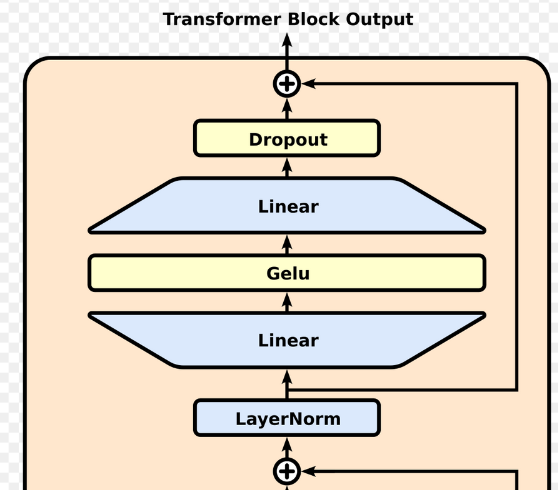
\includegraphics[width=0.4\textwidth]{GeLU.png}
  \end{figure}
}

\frame
{
  \frametitle{Shakesphere Dataset}
  \begin{itemize}
    \item The Shakesphere dataset is a collection of Shakesphere plays.
    \item While it is still large, it is much smaller than the WritingPrompts dataset.
  \end{itemize}
}

\section{Code Explainations}

\frame
{
  \frametitle{Code Explainations}
}

\frame 
{
  \frametitle{Model Recreation with torch.nn.Module}
  \begin{itemize}
    \item Recreated the model with torch.nn.Module under assumption that our code lacks optimization.
    \item With same configuration, original model took 7 hours for 300 epoch, whereas torch.nn.Mudule took 50 minutes for 500 epoch.
    \item Before testing our actual model, we will test the torch.nn.Module model.
  \end{itemize}
}

\frame 
{
  \frametitle{Model Training}
  \begin{itemize}
    \item Trained on 1000 epoch, with learning rate 0.0001.
    \item takes approximately 2 hours to train on rtx 3080.
  \end{itemize}
  \begin{figure}
    \centering
    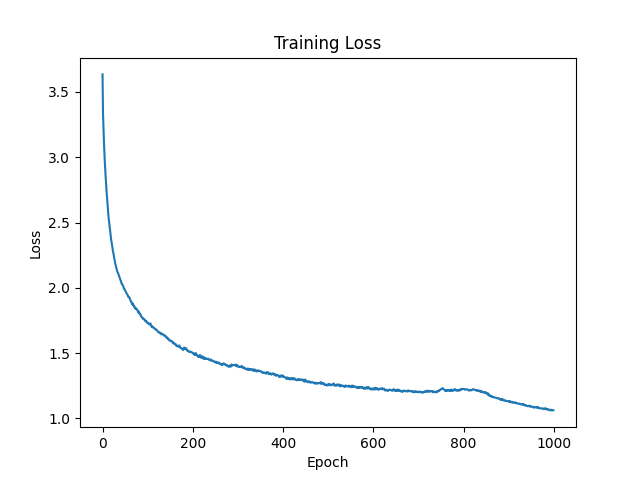
\includegraphics[width=0.6\textwidth]{loss.png}
  \end{figure}
}

% \frame 
% {
%   \frametitle{Sample Generation}
%   \begin{figure}
%     \centering
%     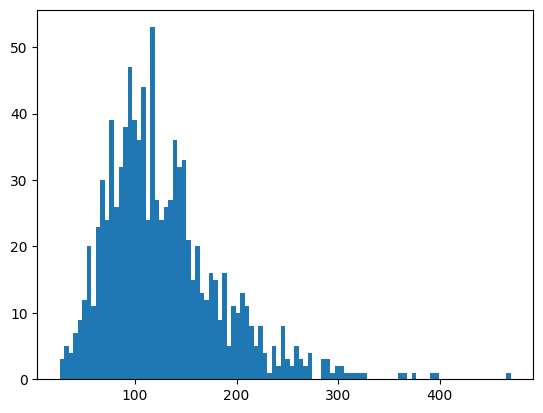
\includegraphics[width=0.6\textwidth]{output_lengths.png}
%   \end{figure}
% }

% \frame
% {
%   \frametitle{Problems}
%   \begin{itemize}
%     \item While we can see decline on loss, it is difficult to have model make coherent sentences.
%     \item The text repeating pattern is caused by Attention mechanism limitation, lack of diversity in training data, and sampling method.
%     \item We should try to implement a probablistic sampling method with temperature.
%   \end{itemize}
% } 

\frame
{
  \frametitle{Remaining Tasks}
  \begin{itemize}
    \item 1. Finish training on the original model.
    \item 2. Implement a probablistic sampling method with temperature.
    \item 3. (If possible) Implement a repetition penalty.
  \end{itemize}
}
\end{document}